\documentclass{beamer}

% This file is a solution template for:

% - Talk at a conference/colloquium.
% - Talk length is about 20min.
% - Style is ornate.


\mode<presentation>
{
  \usetheme{Berlin}
  % or ... Warsaw, Antibes, Bergen, Berkeley

  \setbeamercovered{transparent}
  % or whatever (possibly just delete it)
}


\usepackage[english]{babel}
\usepackage[latin1]{inputenc}

\usepackage{times}
\usepackage[T1]{fontenc}
% Or whatever. Note that the encoding and the font should match. If T1
% does not look nice, try deleting the line with the fontenc.

\usepackage{graphics}

\title[i]{Noise propagation on the Golub-Kahan iterative bidiagonalization
process}
\subtitle{}

\author[Juan Durazo, Brendan Horan, Arthur Mitrano]
{Juan Durazo, Brendan Horan, Arthur Mitrano}
% - Give the names in the same order as the appear in the paper.
% - Use the \inst{?} command only if the authors have different
%   affiliation.

\institute[Arizona State University] % (optional, but mostly needed)
{
  School of Mathematical and Statistical Sciences\\
  Arizona State University}
% - Use the \inst command only if there are several affiliations.
% - Keep it simple, no one is interested in your street address.

\date[APM 520] % (optional, should be abbreviation of conference name)
{April, 2013}
% - Either use conference name or its abbreviation.
% - Not really informative to the audience, more for people (including
%   yourself) who are reading the slides online

\subject{}
% This is only inserted into the PDF information catalog. Can be left
% out. 



% If you have a file called "university-logo-filename.xxx", where xxx
% is a graphic format that can be processed by latex or pdflatex,
% resp., then you can add a logo as follows:

% \pgfdeclareimage[height=0.5cm]{university-logo}{university-logo-filename}
% \logo{\pgfuseimage{university-logo}}



% Delete this, if you do not want the table of contents to pop up at
% the beginning of each subsection:

% If you wish to uncover everything in a step-wise fashion, uncomment
% the following command: 

%\beamerdefaultoverlayspecification{<+->}


\begin{document}

\begin{frame}
  \titlepage
\end{frame}

\begin{frame}{Outline}
  \tableofcontents
  % You might wish to add the option [pausesections]
\end{frame}


% Structuring a talk is a difficult task and the following structure
% may not be suitable. Here are some rules that apply for this
% solution: 

% - Exactly two or three sections (other than the summary).
% - At *most* three subsections per section.
% - Talk about 30s to 2min per frame. So there should be between about
%   15 and 30 frames, all told.

% - A conference audience is likely to know very little of what you
%   are going to talk about. So *simplify*!
% - In a 20min talk, getting the main ideas across is hard
%   enough. Leave out details, even if it means being less precise than
%   you think necessary.
% - If you omit details that are vital to the proof/implementation,
%   just say so once. Everybody will be happy with that.

\section{Introduction}
\subsection{The problem}
\begin{frame}{$Ax=b$}
  \begin{itemize}
    \item We want to solve the problem:
      \begin{equation*}
        Ax=b, \quad A \in \mathbb{R}^{n \times n}, \quad b = b^{exact} + 
        b^{noise}.
      \end{equation*}

    \item $b^{noise}$ is a white noise vector with unknown noise level 
      $\delta_{noise}$.

    \item Information on how the noise propagates can be used to develop 
      a stopping criteria for hybrid methods (iterate and regularize).

    \item The Golub-Kahan iterative bidiagonalization process provides a way to
      analyze how the noise spreads into the core problem.
  \end{itemize}	
\end{frame}
% The idea of this slide is to give an overview of the project, say the reason
% why is important to study the noise propagation into the core problem. The
% main idea is to say that we can develop a stopping criteria for iterative
% methods that are based on the GKIB process, i.e., we can find the iteration
% where we are just adding noise to the solution. Another point that we can add
% is the fact that is possible to recover the noise level without knowing it
% before hand.

\subsection{Golub-Kahan Iterative Bidiagonalization process}
\begin{frame}{Golub-Kahan Iterative Bidiagonalization process}
  \begin{itemize}  
    \item Given $w_{0} = 0$, $s_{1} = b/\beta_{1}$, where $\beta_{1} = \|b\| 
      \neq 0$:
      \begin{align*}
	\alpha_{j}w_{j} &= A^{T}s_{j} - \beta_{j}w_{j-1}, &\quad \|w_{j}\|=1,\\
	\beta_{j+1}s_{j+1} &= Aw_{j} - \alpha_{j}s_{j}, &\quad \|s_{j+1}\|=1
      \end{align*}
      until $\alpha_{j} = 0$ or $\beta_{j+1} = 0$, or we reach the
      dimensionality of the problem.
    
    \item The vectors $s_{k}$ and $w_{k}$ are orthonormal. 
  \end{itemize}
\end{frame}
% Here we should explain that GKIB is a iterative process where we generate a
% basis of orthonormal vectors (s_{k} and w_{k}) and a bidiagonal matrix that
% uses the \alpha_{j}'s and \beta_{j}'s.

\begin{frame}{Matrix form}
  \begin{itemize}
    \item Let $S_{k} = [s_{1},\ldots,s_{k}]$ and $W_{k}= [w_{1},\ldots,w_{k}]$,
      then:
      \begin{equation*}
	A^{T}S_{k} = W_{k}L_{k}^{T}, \quad AW_{k} = [S_{k},s_{k+1}]L_{k+},
      \end{equation*}
      where
      \begin{equation*}
	L_{k} =
	\begin{bmatrix}
	  \alpha_{1} & & & \\
	  \beta_{2} & \alpha_{2} & & \\
	  & \ddots & \ddots & \\
	  & & \beta_{k} & \alpha_{k}
	\end{bmatrix}, \quad
	L_{k+} = 
	\begin{bmatrix}
	  L_{k} \\
	  \beta_{k+1}e_{k}^{T}
	\end{bmatrix}
      \end{equation*}

    \item This bidiagonal decomposition can be used to calculate the SVD of $A$
      in a stable way. $A = S_{k}L_{k}W_{k}^{T} = S_{k}U\Sigma V^{T}W_{k}^{T}$
      $= U_{k}\Sigma V_{k}^{T}$, with $U_{k}$ and $V_{k}$ unitary.
  \end{itemize}
\end{frame}
% Emphasize that after $k$ steps we can write the bidiagonal decomposition,
% which can be used for computing the singular valued decomposition on a stable
% way. Note that product of orthogonal matrices is a orthogonal matrix.

\begin{frame}{Lanczos tridiagonalization of $AA^{T}$}
  \begin{itemize}
    \item Using the starting vector $s_{1} = b/\beta_{1}$, $\beta_{1} = \|b\|$,
      yields in $k$ steps:
      \begin{equation*}
	AA^{T}S_{k} = S_{k}T_{k} + \alpha_{k}\beta_{k+1}s_{k+1}e_{k}^{T},
      \end{equation*}
      and
      \begin{equation*}
	T_{k} = L_{k}L_{k}^{T} = 
	\begin{bmatrix}
	  \alpha_{1}^{2} & \alpha_{1}\beta_{2} & & \\
	  \alpha_{1}\beta_{2} & \alpha_{2}^{2} + \beta_{2}^{2} & \ddots & \\
	  & \ddots & \ddots & \alpha_{k-1}\beta_{k} \\
	  & & \alpha_{k-1}\beta_{k} & \alpha_{k}^{2} + \beta_{k}^{2}
	\end{bmatrix}
      \end{equation*}
      
    \item The matrix $L_{k}$ from the GKIB is a Cholesky factor of the matrix
      $T_{k}$.
  \end{itemize}
\end{frame}
% We just want to mention the connection of Lanczos tridiagonalization with
% GKIB. This will be used later to understand how the noise propagates on the
% $s_{k}$.

\begin{frame}{The core problem}
  \begin{itemize}
    \item Consider $x_{k} = W_{k}y_{k}$ as an approximation for the solution of
      $Ax_{k} \approx b$.

    \item Looking to the residual:
      \begin{align*}
	r_{k} = b - AW_{k}y_{k} &= S_{k+1}(\beta_{1}e_{1} - L_{k+}y_{k}) \\
	&= S_{k}(\beta_{1}e_{1} - L_{k}y_{k}) - 
	(\beta_{k+1}e_{k}^{T}y_{k})s_{k+1},
      \end{align*}
      we get two subproblems:
      \begin{enumerate}
        \item $L_{k}y_{k} = \beta_{1}e_{1}$, for $r_{k}$ orthogonal to $S_{k}$
	  (CGME);
        \item $y_{k} = \min_{y}\|L_{k+}y - \beta_{1}e_{1}\|$, if we minimize 
	  $r_k$ (LSQR or CGLS).
      \end{enumerate}
  \end{itemize}
\end{frame}
% Looking for solutions on the column space of $W_{k}$ lead us to two
% subproblems:
% 1) CGME: residual perpendicular to $S_{k}$;
% 2) CGLS or LSQR: minimization of the residual.
% Here we can quickly describe how from the equation we can get the problems 1
% and 2.

\subsection{Summary}
\begin{frame}{Summarizing}
  \begin{itemize}
    \item The bidiagonalization concentrates the useful information of the
      main problem on its bidiagonal block.
      
    \item In presence of noise, those subproblems might be polluted by the
      noise.

    \item An investigation on how the noise propagates might aid on solving the
      ill-posed problem. (When to stop the iteration procedure).

    \item We will use two main approaches: one looks to the behavior of the
      high frequencies of the vectors $s_{k}$ and the other its normalized
      cumulative periodogram.
  \end{itemize}
\end{frame}
% Summarizing the previous slides and giving a motivation for proceed with the
% study of how the noise propagates through the bidiagonalization process. Here
% we also mention how we going to approach the problem, i.e., using NCP and the
% method of the main reference.

\section{Noise propagation}
\subsection{Picard condition}
\begin{frame}
  \begin{itemize}
    \item The test problem utilized for the numerical experiments was
      \texttt{shaw(400)}, which satisfy the \emph{discrete Picard condition} on
      average.

    \item We used the following noise levels $\delta_{noise} = 10^{-14}, 
      10^{-8}, 10^{-4}$. Where
      \begin{equation*}
	\delta_{noise} = \frac{\|b^{noise}\|}{\|b^{exact}\|}.
      \end{equation*}
  \end{itemize}
\end{frame}
% Introduce the specific problem that will be worked on the numerical
% experiments and remember that the discrete Picard condition hold on average.

\begin{frame}{Picard plot}
  \begin{center}
    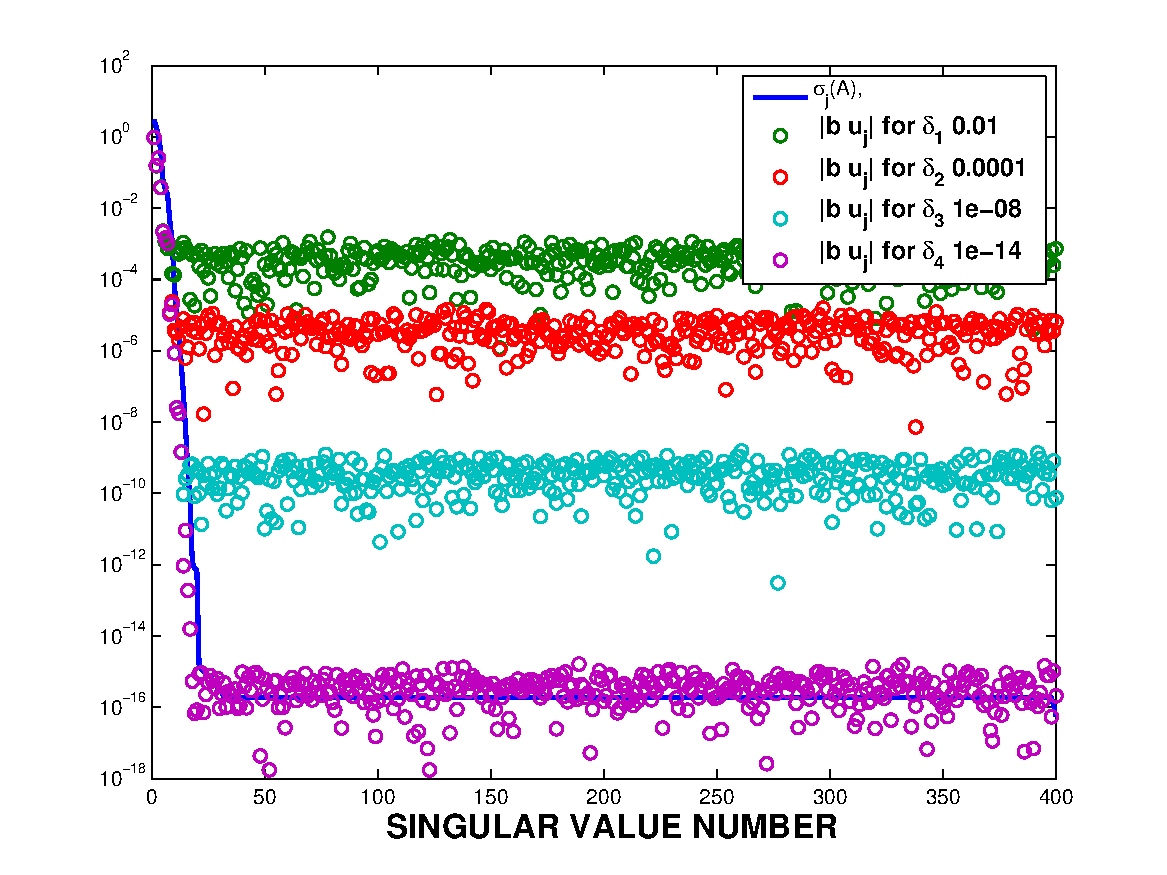
\includegraphics[width=.55\linewidth]{figures/picard}
  \end{center}
  \begin{itemize}
    \item $u_{j}$ are the left singular vectors of $A$.
  \end{itemize}
\end{frame}
% Show that the discrete Picard condition hold until a certain $k$, and then, it
% is drastically violated. Also mention that if we use high precision arithmetic
% the singular values decay faster then the projections $<b,u_{j}>$.

\subsection{Finding $k_{noise}$}
\begin{frame}{Spectral coefficients}
  \begin{center}
    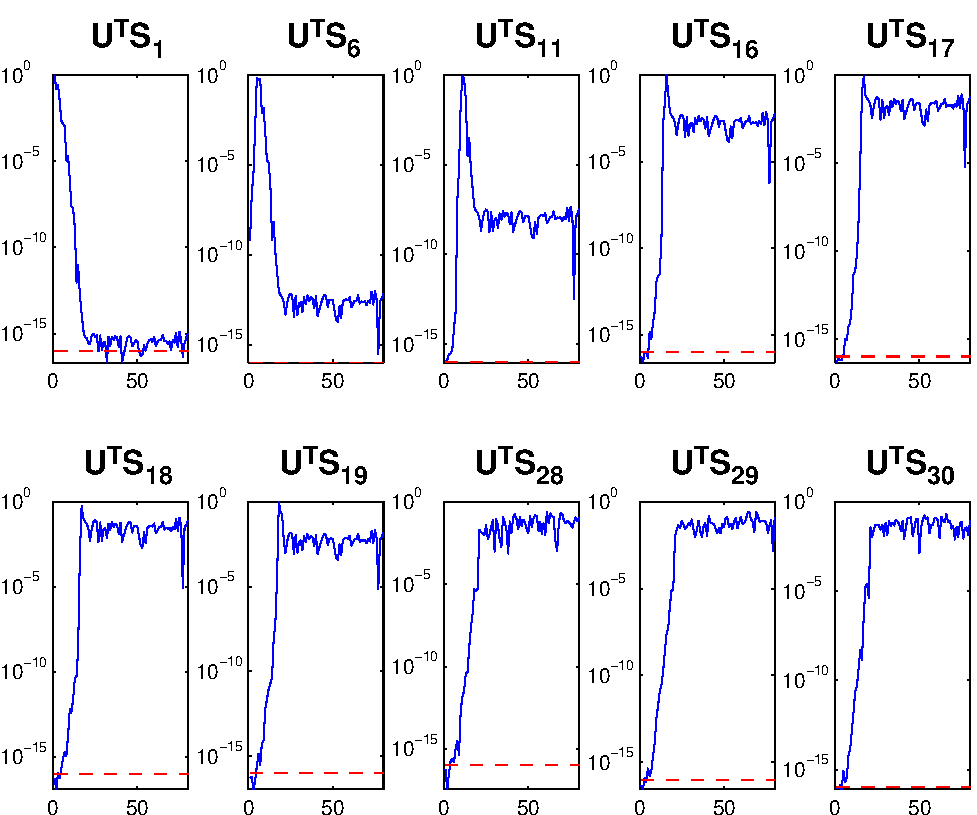
\includegraphics[width=0.55\linewidth]{figures/run1/spec_sk}
  \end{center}
\end{frame}
% Here we want to show that as the we increase $k$ the spectral coefficients
% associated with the lower frequencies singular vectors decay and the ones
% associated with the high frequencies rise and are comparable (this reveals
% the noise).

\begin{frame}{Left singular vectors}
  \begin{center}
    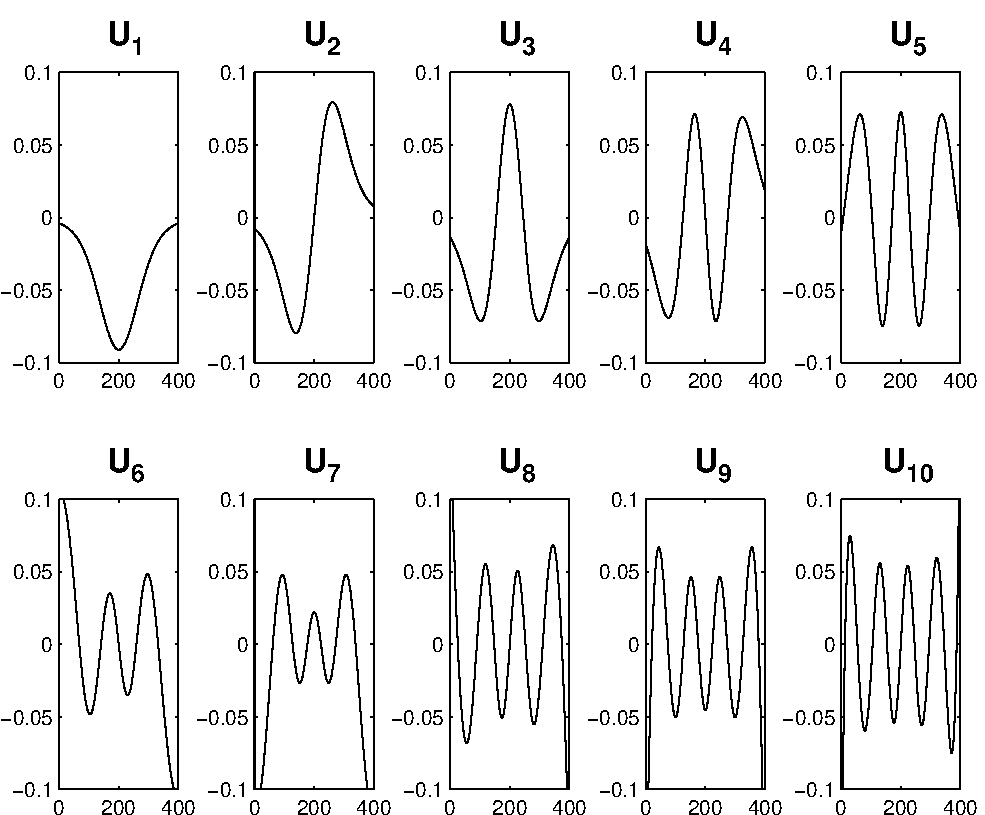
\includegraphics[width=0.55\linewidth]{figures/run1/sing_vecs}
  \end{center}
\end{frame}
% We include the plot of the singular vectors to show that their frequency get
% higher for smaller singular values ($k$ increasing).

\begin{frame}{Analizing the spectral coefficients}
  \begin{itemize}
    \item Using the SVD of $A$ and the Lanczos tridiagonalization of $AA^{T}$:
      \begin{equation*}
	\Sigma^{2}(U^{T}S_{k}) = (U^{T}S_{k})(L_{k}L_{k}^{T}) + 
	\alpha_{k}\beta_{k+1}(U^{T}s_{k+1})e_{k}^{T}.
      \end{equation*}

    \item Setting $k=1$ we can see how the noise spreads to $s_{2}$ (looking to
      the last column):
      \begin{equation*}
	\alpha_{1}\beta_{2}(U^{T}s_{2}) = (\Sigma^{2} - 
	\alpha_{1}^{2}I)U^{T}s_{1}
      \end{equation*}
    
    \item The matrix acts like a filter on the lower frequencies
      \begin{equation*}
	\frac{\sigma_{i}}{\alpha_{1}\beta_{2}} - \frac{\alpha_{1}}{\beta_{2}}
      \end{equation*}
    
    \item $\alpha_{1}/\beta_{2}$ is likely to be larger than $1$.
    \item The noise level on the high frequencies will get larger on $s_{2}$
      than $s_{1}$.
  \end{itemize}
\end{frame}
% Here we should recall the Lanczos tridiagonalization and show how the noise
% spreads to $s_{2}$, i.e., the lower frequencies get smooth (filtered out) and
% the high frequencies get amplified.

\begin{frame}{Generalizing}
  \begin{itemize}
    \item For the general case we can write:
      \begin{equation*}
	U^{T}s_{k+1} = \phi_{k}(\Sigma^{2})U^{T}s_{1}
      \end{equation*}

    \item $\phi_{k}(\lambda)$ is the Lanczos polynomial with root 
      $(\theta_{l}^{(k)})^{2}$, $l = 1,\ldots,k$ (Ritz values).

    \item The large Ritz values $(\theta_{k}^{(k)})^{2}$, 
      $(\theta_{k}^{(k)})^{2}$, \ldots closely approximate the singular values
      $\sigma_{1}^{2}$, $\sigma_{2}^{2}$, \ldots.

    \item Note that the constant term
      \begin{equation*}
	\phi_{k}(0) = \prod_{j=1}^{k}\frac{\alpha_{j}}{\beta_{j+1}} = 
	\rho_{k}^{-1}
      \end{equation*}
  \end{itemize}
\end{frame}
% Here we should explain without many details how what happens from $s_{1}$ to
% $s_{2}$ also happens in general from $s_{1}$ to $s_{k}$ using the Lanczos
% polynomial $\phi_{k}$.

\begin{frame}
  \begin{center}
    %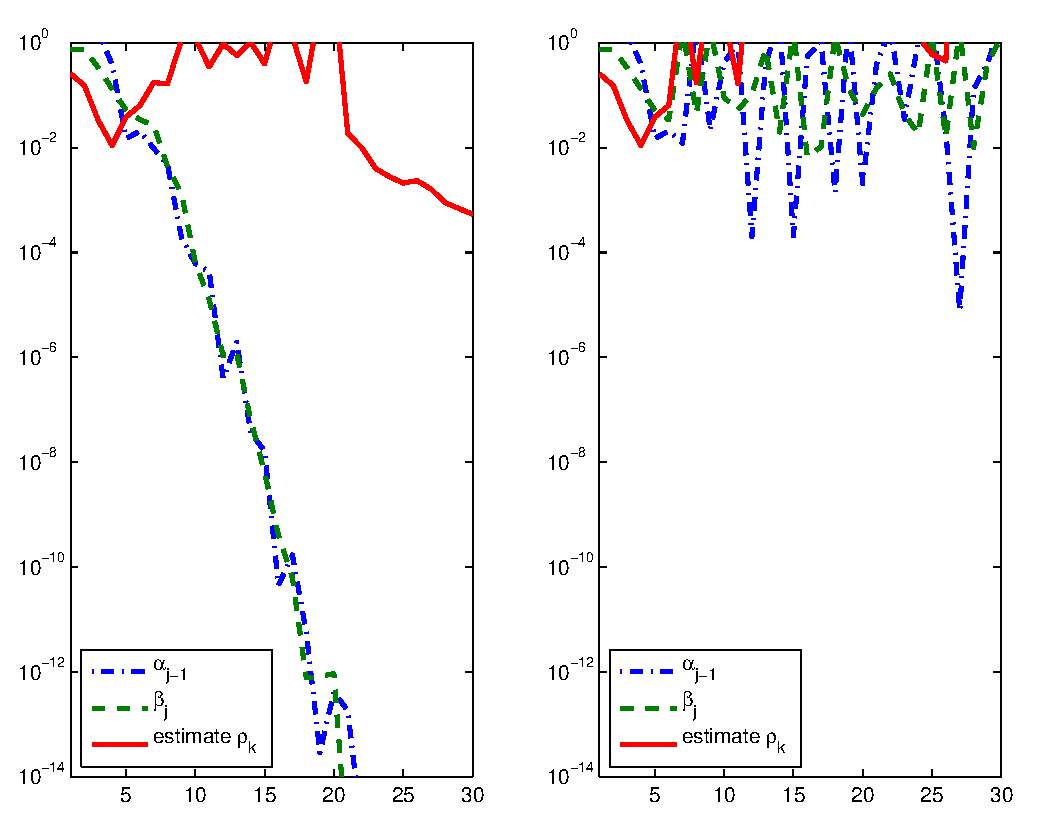
\includegraphics[width=0.35\linewidth]{img/alpha_beta_est}
  \end{center}
  \begin{itemize}
    \item $\phi_{k}$ acts like a filter on low frequencies and the constant term
      $\phi_{k}(0) = \rho_{k}^{-1}$ causes the amplification of the high
      frequency noise present in the noisy vector $s_{1}$.
  \end{itemize}
\end{frame}
% The idea here is to show in the graph that $\rho_{k}$ is increasing and
% summarize how the noise is being spread, i.e., being filter out on the lower
% frequencies and amplified on the higher ones.

\begin{frame}{Signal and noise spaces}
  \begin{center}
    %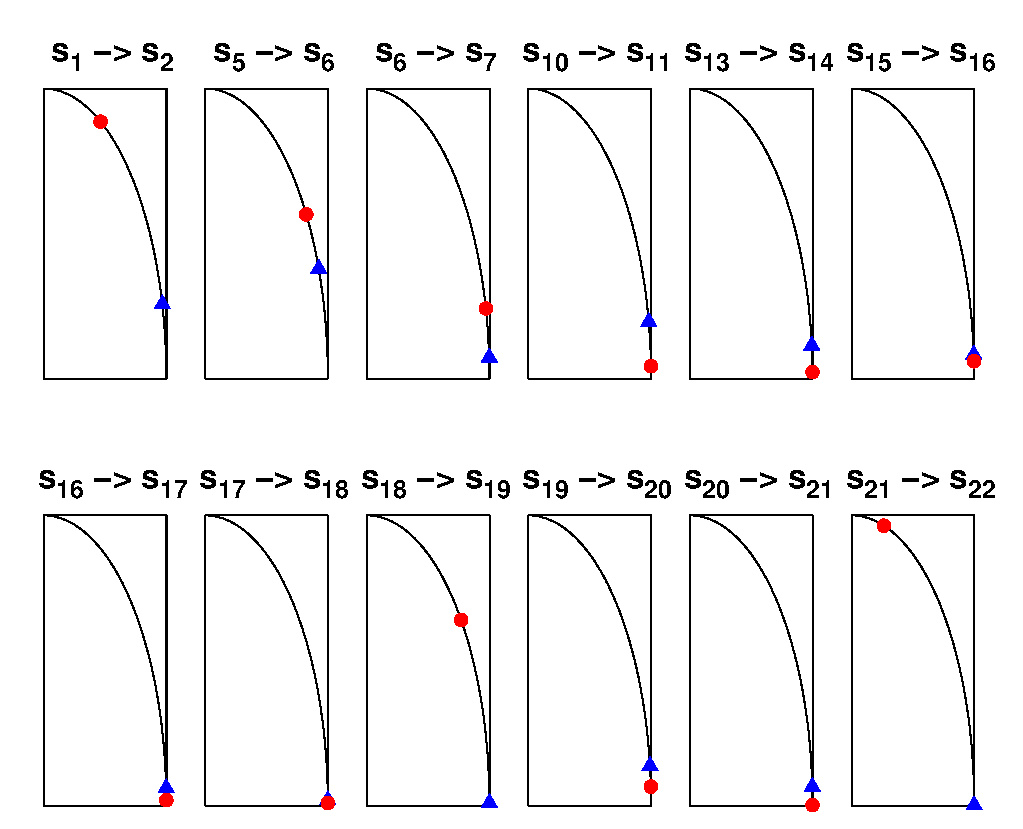
\includegraphics[width=0.35\linewidth]{img/signal_noise_space}
  \end{center}
  \begin{itemize}
    \item $span\left\{u_{1},\ldots,u_{k+1}\right\}$ is the signal subspace.
    \item $span\left\{u_{k+2},\ldots,u_{n}\right\}$ is the noise subspace.
  \end{itemize}
\end{frame}
% Explain the plot and give a reasoning why it it reveals the noise. Note that
% the vectors are moving counterclockwise (approaching the noise subspace) and
% then there is an iteration where one of them move clockwise (approaching the
% signal subspace), indicating that $k_{noise} + 2 = 19$, i.e., $k_{noise} = 17$

\subsection{Behavior of $s_{k}^{exact}$ and $s_{k}^{noise}$}
\begin{frame}{Behavior of $s_{k}^{exact}$ and $s_{k}^{noise}$}
  \begin{itemize}
    \item To further illustrate the noise amplification we look to
      $s_{k}^{exact}$ and $s_{k}^{noise}$. Let $s_{1} = s_{1}^{exact} + 
      s_{1}^{noise}$ and
      \begin{align*}
	\beta_{k+1}s_{k+1}^{exact} &= Aw_{k} - \alpha_{k}s_{k}^{exact}, \\
	\beta_{k+1}s_{k+1}^{noise} &= -\alpha_{k}s_{k}^{noise}, \\
	s_{k+1} &= s_{k+1}^{exact} + s_{k+1}^{exact}, \quad 
	\beta_{k+1}s_{k+1} = Aw_{k} - \alpha_{k}s_{k}.
      \end{align*}
      
    \item They aren't the true exact and noise data, but they give good
      approximations to the euclidean norm. See \cite{bidiagonalization}.

    \item Note that,
      \begin{equation*}
	s_{k+1}^{noise} = -\frac{\alpha_{k}}{\beta_{k+1}}s_{k}^{noise} =
	(-1)^{k}\rho_{k}^{-1}s_{1}^{noise}.
      \end{equation*}
  \end{itemize}
\end{frame}
% Here we going to just say we are using the definition of \cite{bidiagonal} and
% present the plots on the next slides. Make sure to mention that this
% definition do not give the exact and noise true data, however it is a good
% approximation for the euclidean norm of those.

\begin{frame}{$s_{k}$ plots}
  \begin{center}
    %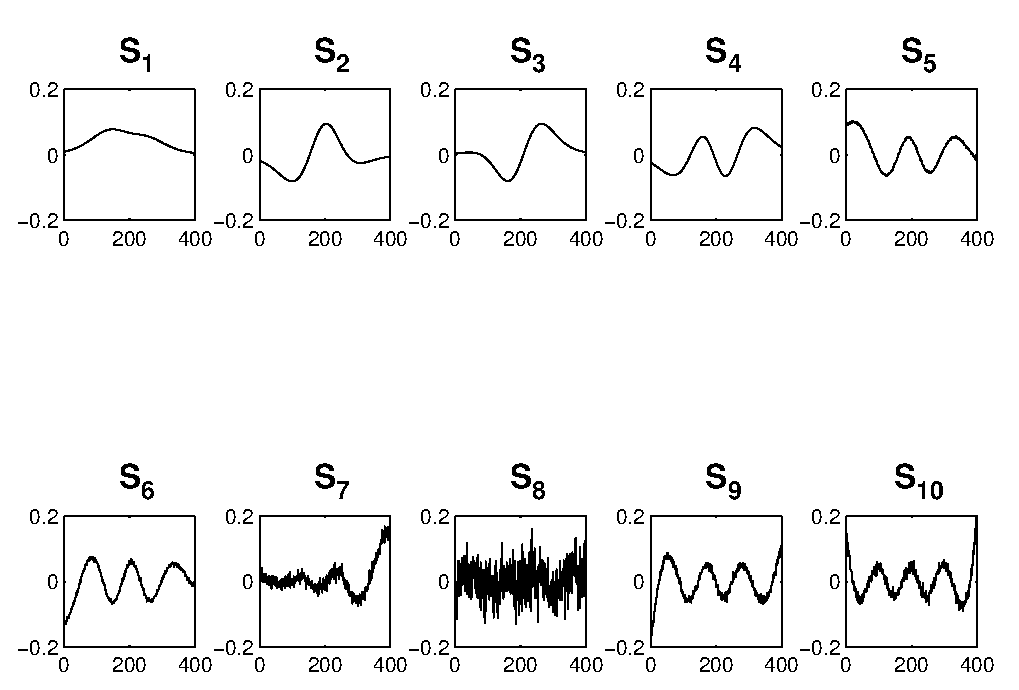
\includegraphics[width=0.35\linewidth]{img/sk_plots}
  \end{center}
\end{frame}

\begin{frame}{$s_{k}^{exact}$ plots}
  \begin{center}
    %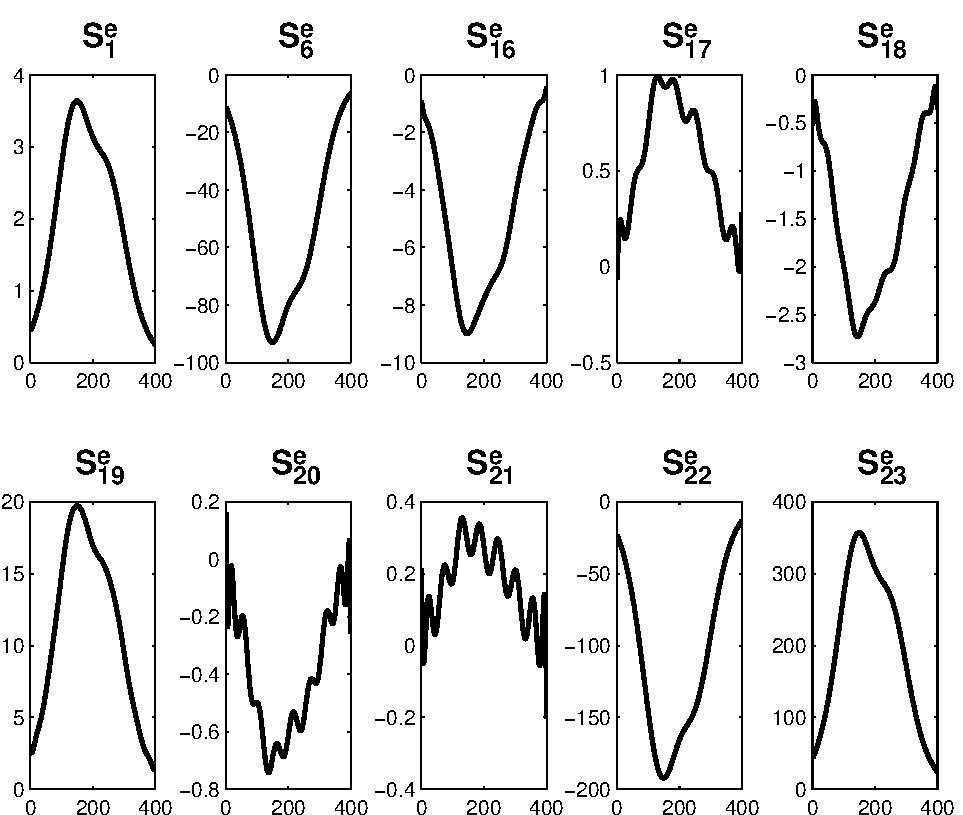
\includegraphics[width=0.35\linewidth]{img/exact_parts}
  \end{center}
\end{frame}

\begin{frame}{$s_{k}^{noise}$ plots}
  \begin{center}
    %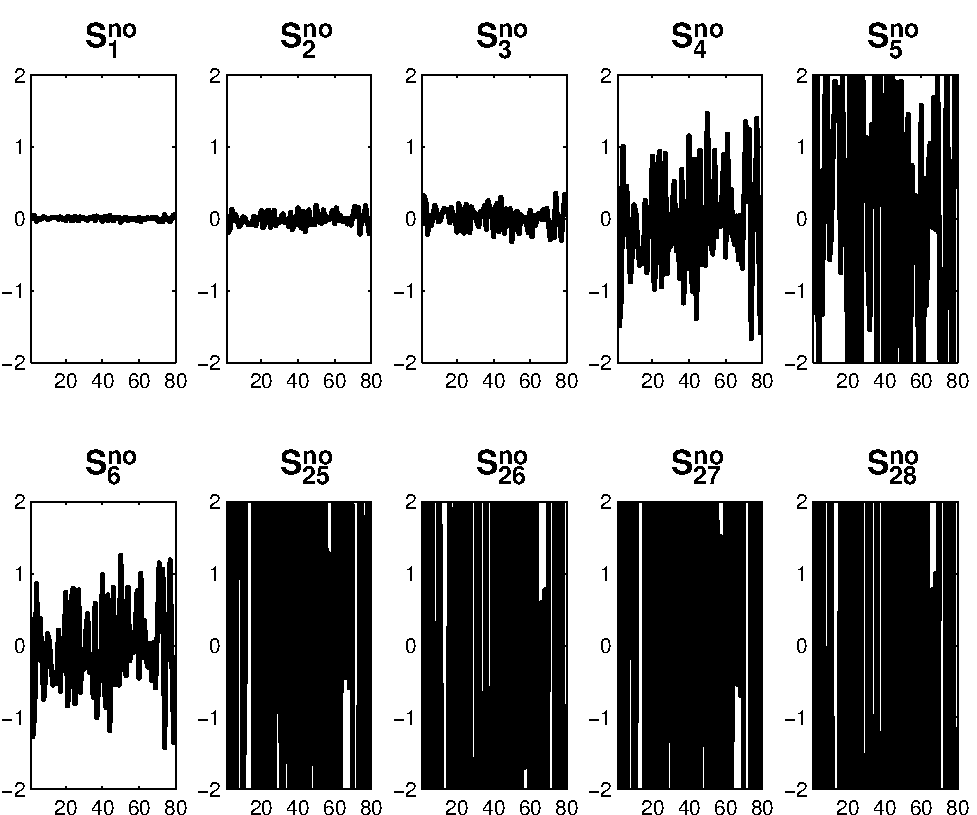
\includegraphics[width=0.35\linewidth]{img/noise_parts}
  \end{center}
\end{frame}

\begin{frame}{Other ways to find $k_{noise}$}
  \begin{itemize}
    \item Is possible to use other basis, like Fourier basis. This allows FFT.
      \begin{center}
        %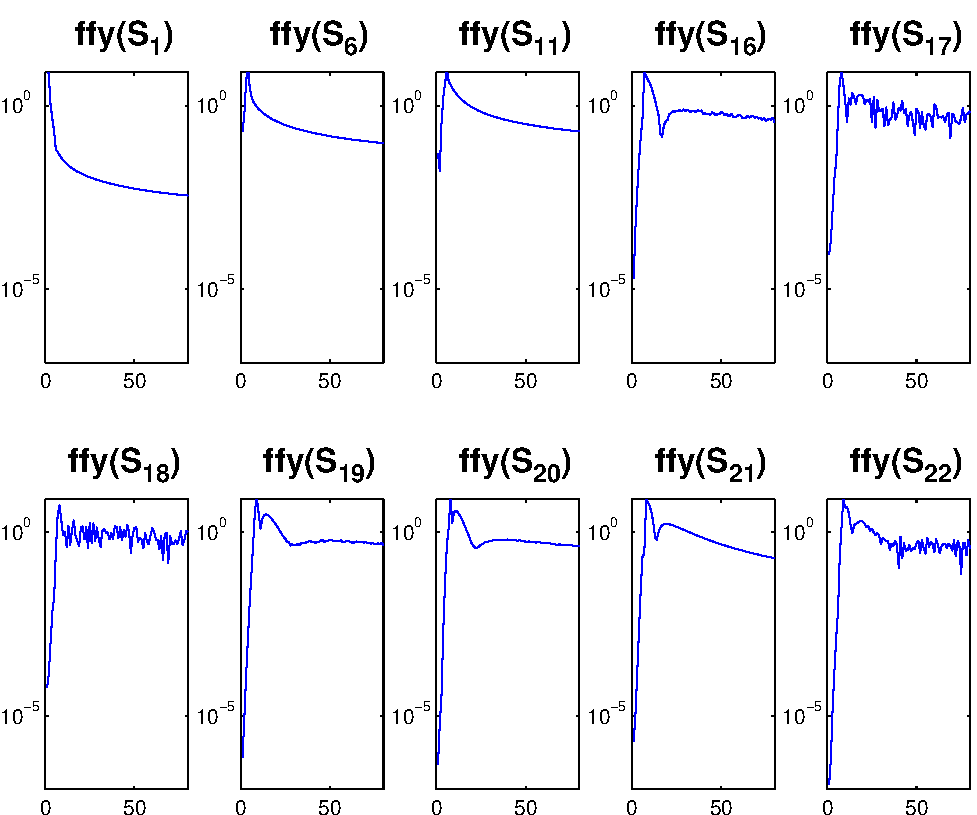
\includegraphics[width=0.35\linewidth]{img/fft_sk}
      \end{center}
  \end{itemize}
\end{frame}

\subsection{More theory}
\begin{frame}{$k_{noise}$ and $\delta_{noise}$}
  \begin{itemize}
    \item It is possible to find $k_{noise}$ \emph{without} using spectral
      decomposition.
    \item To find find the noise level we used
      \begin{equation*}
	\delta_{noise} \approx \frac{1}{2}\rho_{k_{noise}}.
      \end{equation*}
    \item We refer \cite{bidiagonalization} for more details.
  \end{itemize}
\end{frame}


\subsection{Normalized Cumulative Periodogram}
\begin{frame}{Normalized Cumulative Periodogram (NCP)}
  \begin{itemize}
    \item Definition:
      \begin{equation*}
	\mathbf{c}_{j} = |dft(\mathbf{y})_{j}|^{2}, \quad z_{j} =
	\frac{\sum_{i=1}^{j}\mathbf{c}_{i}}{\sum_{i=1}^{q}\mathbf{c}_{i}},
	\quad j = 1,\ldots,q.
      \end{equation*}

    \item Kolmogorov-Smirnoff at $5\%$ significance level: the NCP curve must
      lie between the limits $\pm 1.35q^{-1/2}$ of the straight line (diagonal).

    \item There are other kind of measures for testing if a distribution is
      white-noise like, e.g., \emph{total deviation}.
    \end{itemize}
\end{frame}
% Talk about the NCP definition of a vector $\mathbf{y}$, the $\mathbf{c}_{j}$
% are components of the power spectrum $\mathbf{c}$.
% After explain the K-S test make sure that you mention that are other possible
% ways to measure if a distribution is white-noise like. This is more a
% statistical thing.

\begin{frame}{NCP plot}
  \begin{center}
    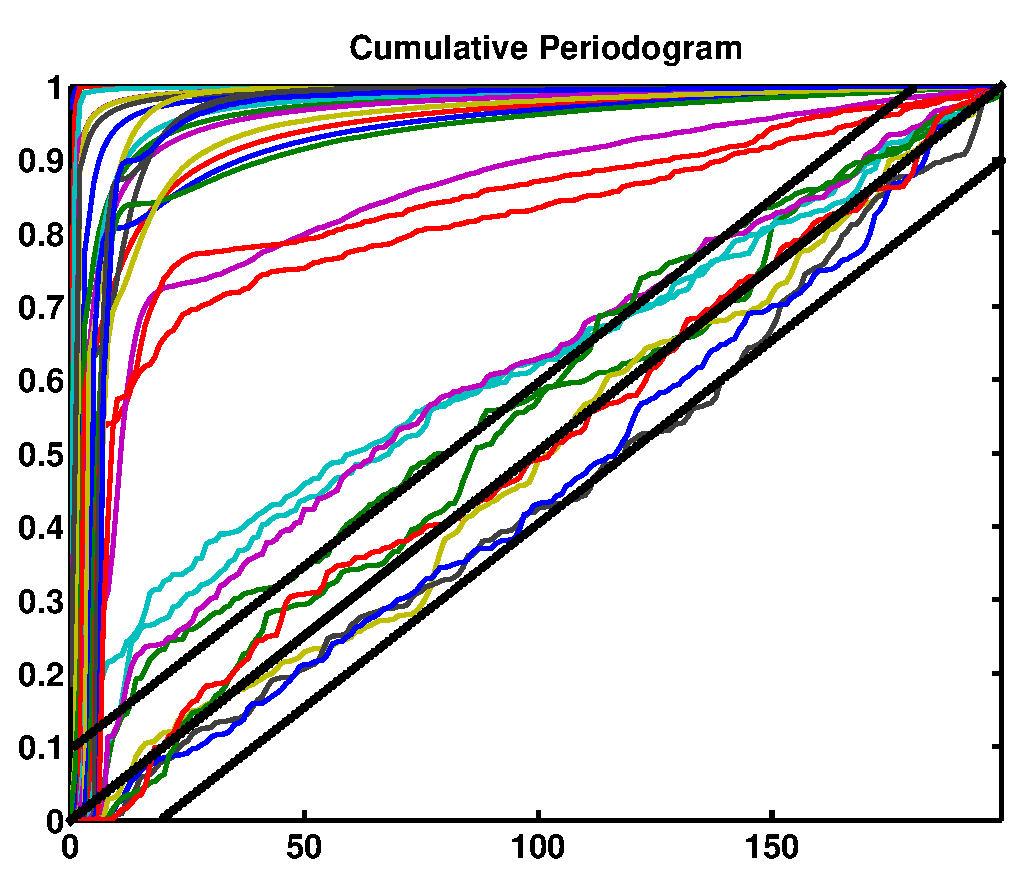
\includegraphics[width=0.55\linewidth]{figures/run1/cum_per}
  \end{center}
\end{frame}
% Remember to explain the frequency idea, i.e., why the graphs have a S-shape.

\begin{frame}{White-noise measures}
  \begin{center}
    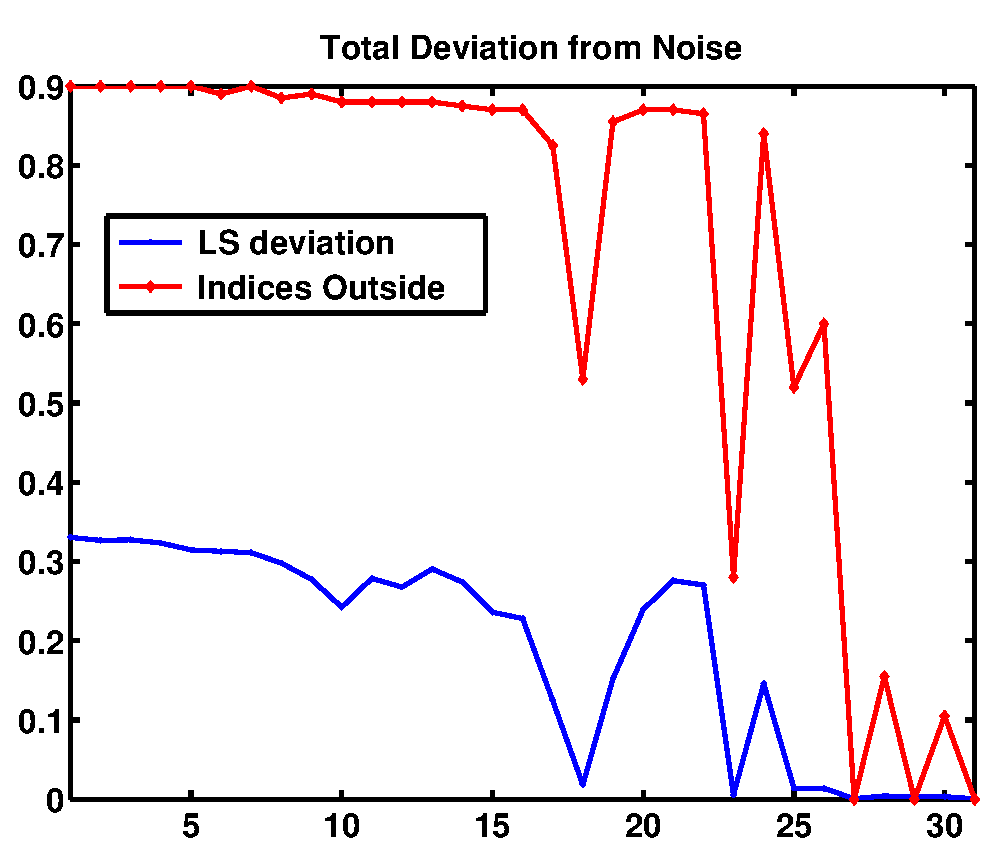
\includegraphics[width=0.55\linewidth]{figures/run1/total_deviation}
  \end{center}
\end{frame}
% Here we must emphasize that both methods indicate that the vectors become
% white-noise like at the same time. As the advantage of the NCP method we
% should mention that it is a much simpler concept to understand.

\subsection{NCPs vs ``GKIB''}
\begin{frame}{Comparing the methods to find $k_{noise}$}
  \begin{center}
    \begin{tabular}{l||c|c|c|c}
      \multicolumn{1}{l||}{problem} & \multicolumn{4}{l}{\texttt{shaw(400)}} \\
      \hline \hline 
      $\delta_{noise}$ & $10^{-14}$ & $10^{-8}$ & $10^{-4}$ & $10^{-2}$ \\
      \hline
      $k_{noise}$ (GKIB) & $17$ & $11$ & $7$ & $3$ \\
      \hline
      $k_{noise}$ (NCP) & $27$ & $26$ & $8$ & $23$ \\
      \hline
      $\tilde{\delta}_{noise}$ (GKIB) & $5.9E-15$ & $1.2E-8$ & $5.3E-5$ &
      $1.6E-2$ \\
      \hline
      $\tilde{\delta}_{noise}$ (NCP) & $1.5E-15$ & $8.1E-9$ & $3.7E-4$ & 
      $3.6E-3$ \\
    \end{tabular}
  \end{center}
  \begin{itemize}
    \item $\tilde{\delta}_{noise}$ indicates the estimated noise level.
    \end{itemize}
\end{frame}
% Go over the results of the table making comparisons and interpreting the
% results. As the advantage of the NCP method we should mention that it is a 
% simpler concept to understand.

\begin{frame}{Spectral coefficients with higher precision}
  \begin{center}
    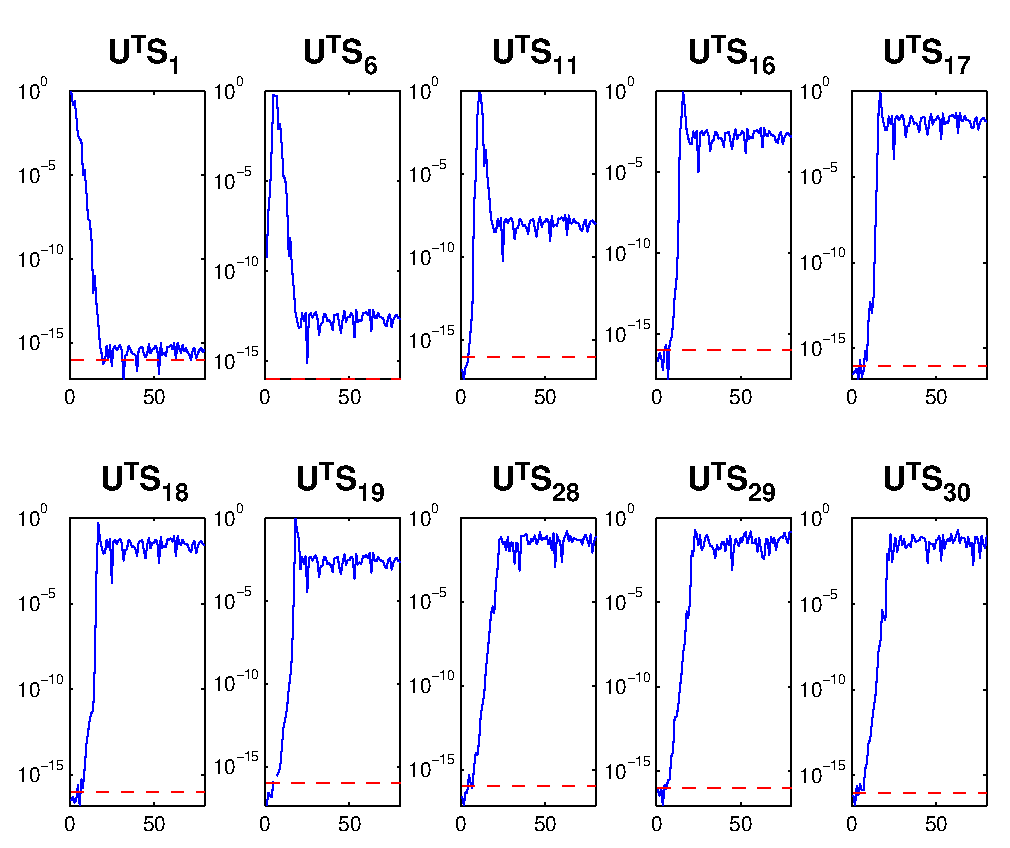
\includegraphics[width=0.55\linewidth]{figures_shawvpa/run1/spec_sk}
  \end{center}
\end{frame}


\begin{frame}{Comparing the methods to find $k_{noise}$ with higher precision}
  \begin{center}
    \begin{tabular}{l||c|c|c|c}
      \multicolumn{1}{l||}{problem} & \multicolumn{4}{l}{\texttt{shaw(400)}} \\
      \hline \hline 
      $\delta_{noise}$ & $10^{-14}$ & $10^{-8}$ & $10^{-4}$ & $10^{-2}$ \\
      \hline
      $k_{noise}$ (GKIB) & $17$ & $12$ & $7$ & $4$ \\
      \hline
      $k_{noise}$ (NCP) & $26$ & $26$ & $26$ & $26$ \\
      \hline
      $\tilde{\delta}_{noise}$ (GKIB) & $1.2E-14$ & $5.7E-9$ & $5.5E-3$ &
      $1.6E-2$ \\
      \hline
      $\tilde{\delta}_{noise}$ (NCP) & $2.0E-15$ & $1.1E-9$ & $1.5E-6$ & 
      $3.7E-4$ \\
    \end{tabular}
  \end{center}
  \begin{itemize}
    \item $\tilde{\delta}_{noise}$ indicates the estimated noise level.
    \end{itemize}
\end{frame}



\section{Resolution matrix}
\subsection{Expresion for $R^{\sharp}$}
\begin{frame}{Resolution matrix of the GKIB process}
  \begin{itemize}
    \item $R^{\sharp} = W_{k}(L_{k}^{T}L_{k})^{-1}L_{k}^{T}S_{k}^{T}A$.
    \item Show the resolution matrix in Matlab.
    \end{itemize}
\end{frame}
% Explain what is a resolution matrix and why it is important during the
% presentation using Matlab.

\begin{thebibliography}{1}
  \bibitem{bidiagonalization}  Hnetynkova, I. and Plesinger, M.. 
    \emph{The regularizing effect of the Golub-Kahan iterative bidiagonalization 
      and revealing the noise level in the data.}
      BIT Numer Math (2009) 49: 669-696.
\end{thebibliography}

\end{document}
